\subsection{Opis hipotezy}\label{opis-hipotezy}

\textbf{Numer:} 6\\\textbf{Nazwa:} Przekraczanie prędkości a
czas\\\textbf{Treść:} Rzadziej wypadki spowodowane przekroczeniem
prędkości przez kierowcę będą zdarzać się w zimie i na jesień niż w
pozostałych porach roku, gdyż kierowcy są ostrożniejsi w trudniejszych
warunkach.

\subsection{Wyniki związane z
hipotezą}\label{wyniki-zwiazane-z-hipoteza}

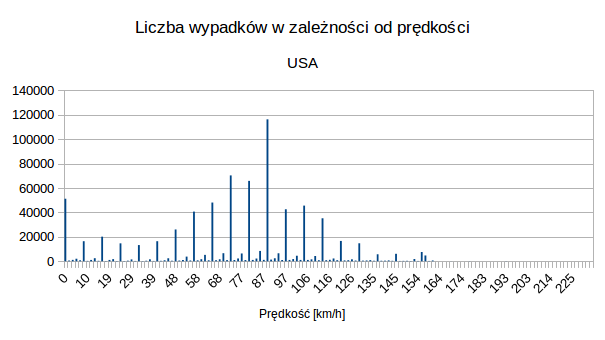
\includegraphics[width=0.8\textwidth]{images/hipotheses/speed/speed.png}

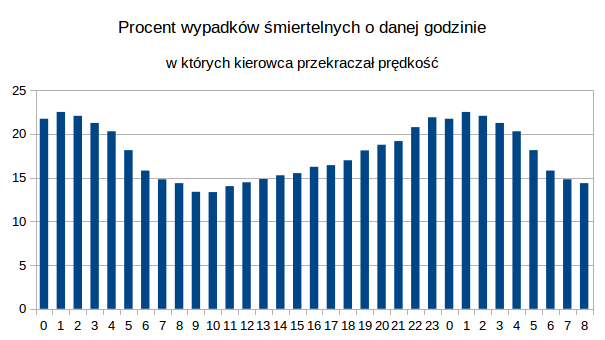
\includegraphics[width=0.8\textwidth]{images/hipotheses/speed/speed_exceeded_by_hour.png}

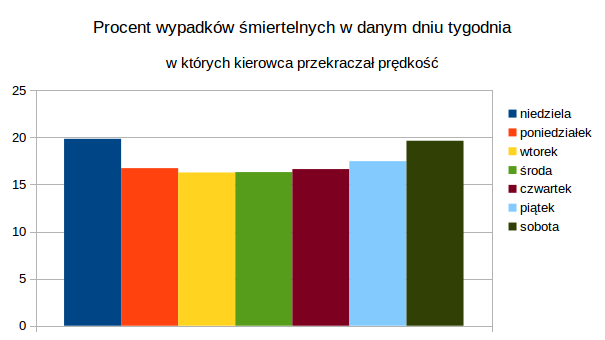
\includegraphics[width=0.8\textwidth]{images/hipotheses/speed/speed_exceeded_by_day_of_week.png}

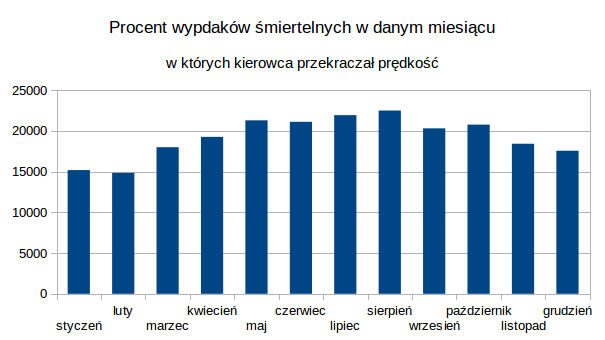
\includegraphics[width=0.8\textwidth]{images/hipotheses/speed/speed_exceeded_by_month.png}

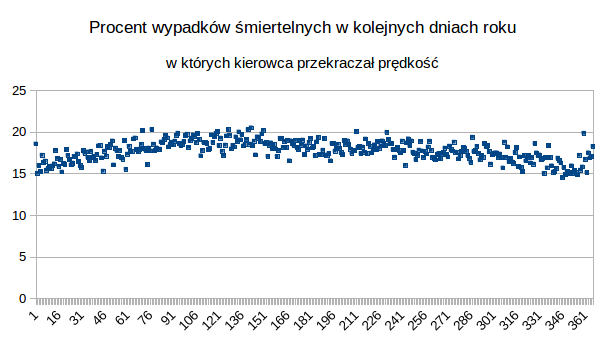
\includegraphics[width=0.8\textwidth]{images/hipotheses/speed/speed_exceeded_by_day_of_year.png}

\subsection{Weryfikacja i wnioski}\label{weryfikacja-i-wnioski}

Hipoteza potwierdziła się. Patrząc na wykres w zależności od miesiąca
oraz dnia w roku, najmniej wypadków związanych z przekroczeniem
prędkości obserwujemy w miesiącach zimowych (styczeń, luty, grudzień).
Kierowcy z mniejszą brawurą podchodzą do jazdy w trudniejszych warunkach
i rzadziej łamią wtedy przepisy.

Większa brawura kierowców wychodzi w weekendy, wartości procentowe w
sobotę i niedzielę przekraczają o blisko 5 procent pozostałe dni.

Ciekawa jest także zależność liczby wypadków od prędkości. Widać, że
największa wartość przypada na 90 km/h.
